\section{Our Construction}\label{sec:construction}



\subsection{Overview}
First we describe our join algorithm without any privacy and then we will discuss how this translates to the secret shared setting. \figureref{fig:mapping} depicts our algorithm with the following phases:
\begin{enumerate}
	\item \label{step:overview1}  $Y$ is inserted into a cuckoo hash table $\ytable$ based on the join-key(s). That is, let us assume the columns $Y_1$ and $X_1$ are the join keys. Then 
	row $Y[i]$ is inserted at $\ytable[j]$ for some $j\in \{h_0(Y_1[i]), h_1(Y_1[i])\}$.
	\item \label{step:overview2} Each row $X[i]$ needs to be compared with the rows $\ytable[j]$ for $j\in \{h_0(X_1[i]), h_1(X_1[i])\}$. As such, $\ytable[h_0(X_1[i])]$ is mapped to a new row $\widehat{Y}^0[i]$ and $\ytable[h_1(X_1[i])$ to $\widehat{Y}^1[i]$. 
	\item \label{step:overview3} It is now the case that if row $X[i]$ has a machining key in $Y$, then this row will be located at $\widehat{Y}^0[i]$ or $\widehat{Y}^1[i]$. As such, these rows can directly be compared to determine if there is a match on the join keys and the where clause evaluates to true. Let $b_i=1$ if there is such a match and $0$ otherwise.
	\item \label{step:overview4} Various types of joins can then be constructed from locally comparing row $i$ from these tables, i.e. $X[i],\widehat{Y}^0[i], \widehat{Y}^1[i]$. For example, an inner join is constructed from all the rows where $b_i=1$ by selecting the values from $X[i]$ and either $\widehat{Y}^0[i]$ or $\widehat{Y}^1[i]$ depending on which one matches. If there is no match, then that output row is set to \Null.
\end{enumerate} 

\begin{figure}\centering
	\frame{	\begin{tikzpicture}[scale=0.48, every node/.style={scale=0.48}]
		\draw (0, 0) node[inner sep=0] {{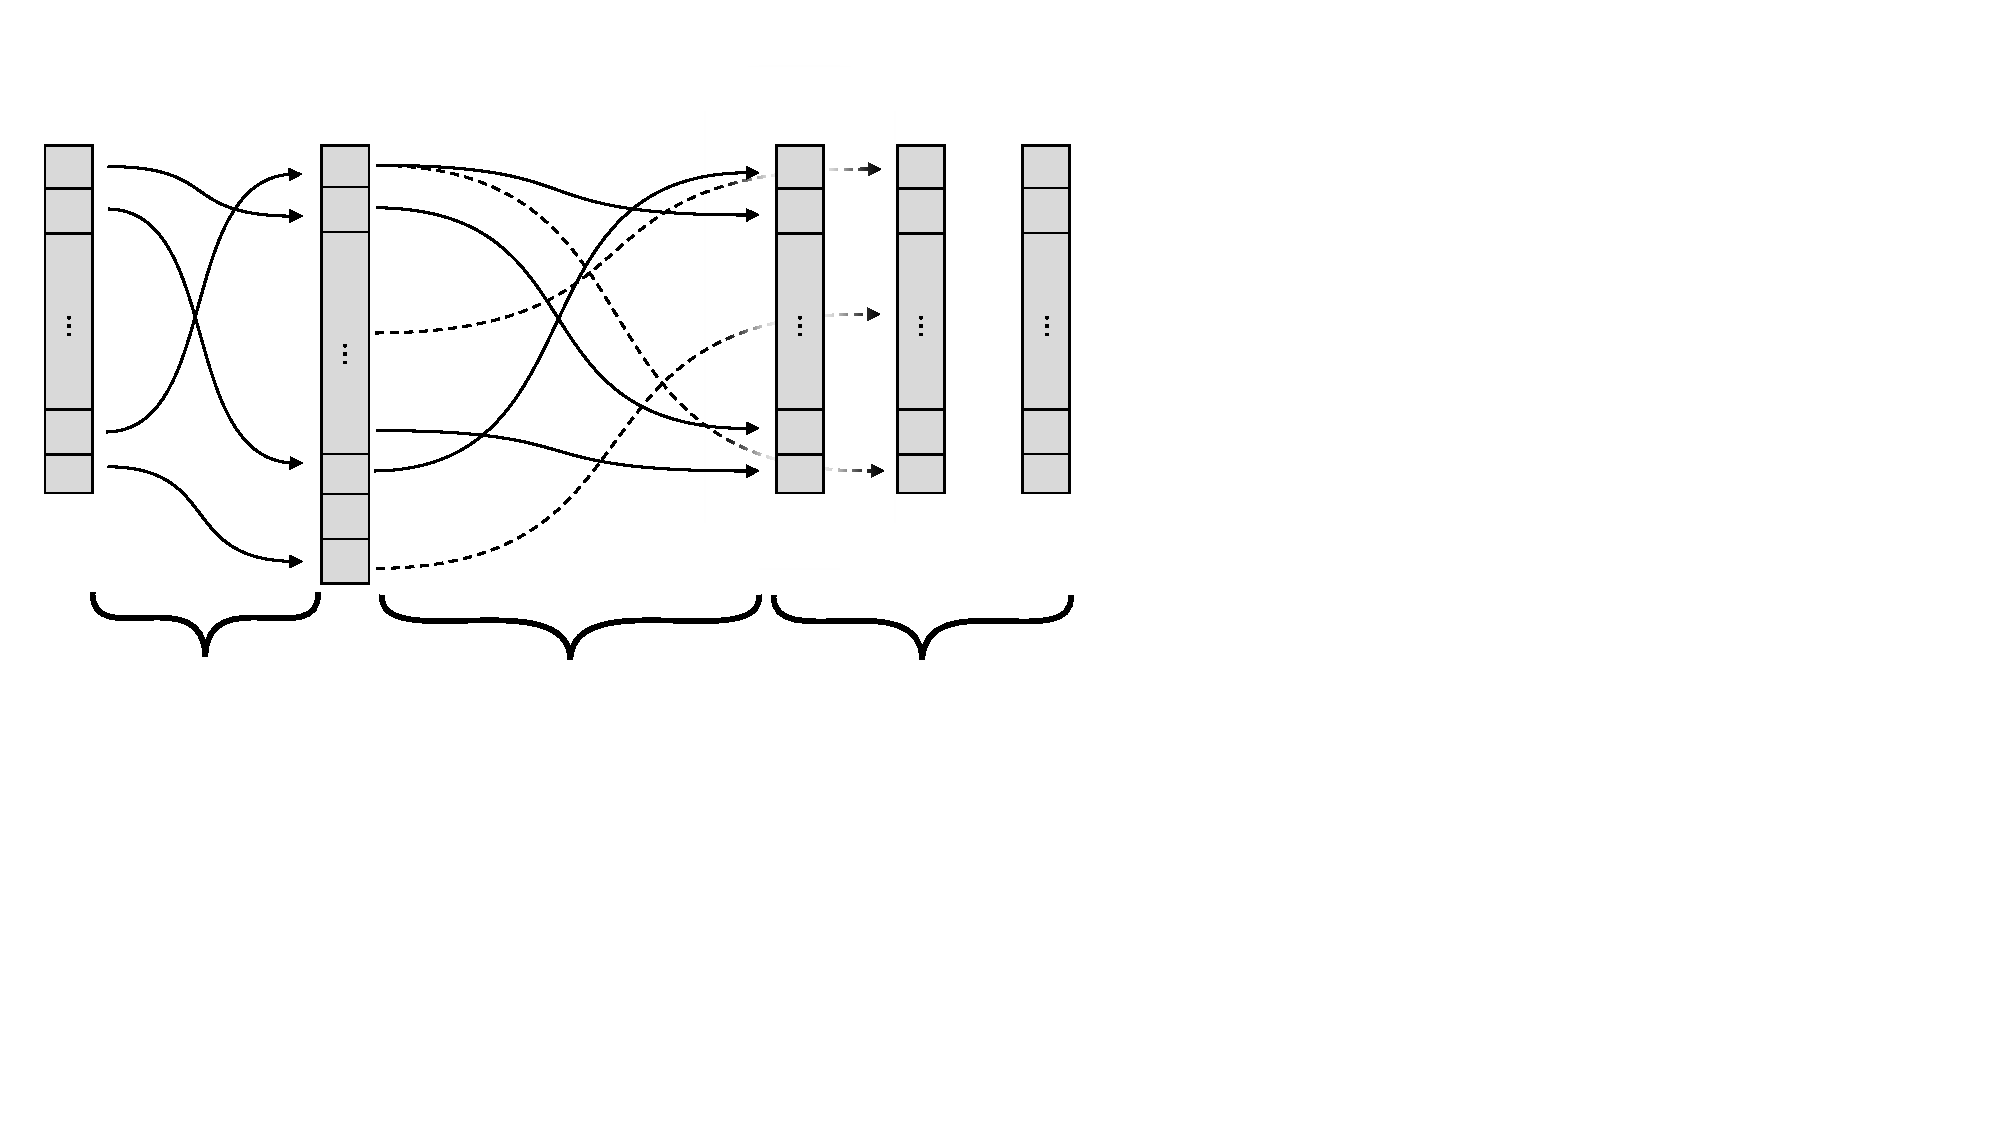
\includegraphics[trim={0cm 7cm 14cm 1cm},clip,width=\textwidth]{diga.pdf}}};
		\draw (-7.9cm,4cm) node {\large$\share{Y}$};
		\draw (7.2cm,4cm) node {\large$X$};
		\draw (-3.7cm,4cm) node {\large$\ytable=\textsf{Cuckoo}(Y)$};
		%	\draw (3.8cm,4.6cm) node {\large Selections w/ $h_0(x),h_1(x)$};
		\draw (3.3cm,4cm) node { \large$\widehat{Y}^0$};
		\draw (5.2cm,4cm) node { \large$\widehat{Y}^1$};
		
		\draw (-5.8cm,-4.5cm) node { 1) Cuckoo hash  $Y$  };
		\draw (-5.8cm,-5.0cm) node { using oblv. permutation.};
		\draw (-5.8cm,-5.5cm) node { $\exists j$ s.t. $T[h_j(Y[i])]=Y[i]$. };
		
		
		\draw (-0.3cm,-4.5cm) node { 2) Select Cuckoo locations $T[h_j(X[i])]$  };
		\draw (-0.3cm,-5.0cm) node { using oblv. switching network.};
		\draw (-0.3cm,-5.5cm) node { $\widehat{Y}^j[i]=T[h_j(X[i])]$.};
		
		
		
		\draw (5.4cm,-4.5cm) node { 3) Compare $\widehat{Y}^0[i],\widehat{Y}^1[i]$ w/ $X[i]$};
		\draw (5.4cm,-5.0cm) node { using MPC circuit and  };
		\draw (5.4cm,-5.5cm) node {construct output row. };
		\end{tikzpicture}}
	\vspace{-0.3cm}
	\caption{Overview of the join protocol using oblivious switching network.\label{fig:mapping}}
	\vspace{-0.4cm}
\end{figure}

The main challenge in bringing the described algorithm to the secret shared setting is constructing the cuckoo hash table $\ytable$ and selecting rows from $\ytable$ without leaking sensitive information. We achieve this with the use an MPC friendly \emph{randomized encoding} and a new three-party protocol called an \emph{oblivious switching network}.


Let us continue to assume that the columns $X_1$ and $Y_1$ are the join-keys. Our protocol begins by generating a \emph{randomized encoding} for each of the secret shared join-key $\share{x_i}\in \share{X_1}$ and $ \share{y_i}\in \share{Y_1}$. \figureref{fig:randomized-encode-ideal} contains the ideal functionality for this encoding which takes secret shares from the parties, apply a PRF $F_k$ to the reconstructed value using a internally sampled key $k$, and returns the resulting value to one of the three parties. For $\share{ x_i}:= \share{X_1}[i]$, \Party{0} will learn $F_k(x_i)$ while \Party{1} will learn $F_k(y_i)$ for $\share{ y_i}:=\share{Y_1}[i]$. Since the join-keys $x_i$ (resp. $y_i$) are unique and $k$ is not known, this can be simulated by sending random values to \Party{0} (resp. \Party{1}).

Party \Party{1} proceeds by constructing a \emph{secret shared} cuckoo hash table $\shareTwo{\ytable}$ from the rows of $\share{Y}$ where the hash function values for row $i$ are defined as $h_j(y_i) = H( j || F_k(y_i))$. Note that \Party{1} knows only the randomized encodings $F_k(y_i)$ of each row $Y[i]$, and not the contents of the row itself. The goal in this step is to construct a secret shared cuckoo table $\shareTwo{\ytable}$ such that row $Y[i]$ is located at $\ytable[h_j(y_i)]$ for some $j$. We construct  $\shareTwo{\ytable}$ using a three-party \emph{oblivious permutation protocol} where \Party{1} inputs a permutation $\pi$, all parties input secret shares of $Y$, and the result is secret shares of ``$Y$ permuted according to $\pi$'' which forms $\ytable$ (details follow later). This completes \stepref{step:overview1} and is the first transformation shown in \figureref{fig:mapping}.

It is now the case that $\shareTwo{\ytable}$ is a valid cuckoo hash table of $\share Y$ which is secret shared between \Party{0} and \Party{1}. Party \Party{0}, who knows the randomized encodings $F_k(x_i)$ for all $\share{ x_i}:= \share{X_1}[i]$, now must compare the rows of $\shareTwo{\ytable}$ indexed by $h_j(x_i)= H( j || F_k(x_i))$ with the row $\share X[i]$. In particular, assuming we use two cuckoo hash functions, then \Party{0} constructs two \emph{oblivious switching networks} that maps the shares $\shareTwo{\ytable[{h_0(x_i)}]}$ and $\shareTwo{\ytable[{h_1(x_i)}]}$ to be ``aligned" with $\share X[i]$. Exactly how such a network operates is discussed later but the result is two new tables $\shareTwo{\widehat{Y}^0},\shareTwo{\widehat{Y}^1}$ such that $\ytable[{h_j(x_i)}]=\widehat{Y}^j[i]$. This completes \stepref{step:overview2} and is the second transformation shown in \figureref{fig:mapping}.

Once the shares of $\widehat{Y}^0[i]={\ytable[{h_0(x_i)}]}, \widehat{Y}^1[i]={\ytable[{h_1(x_i)}]}$ are obtained using the switching network, the parties employ an MPC protocol to directly compare these rows with $\share{X}[i]$. That is, they compute a bit $\share{b}$ which equals one if the join-keys are equal and the \texttt{where} clause $P(\shareTwo{\widehat{Y}^j}[i],\share{X}[i])$ outputs one for some $j$. For each row, the output row for an inner join is constructed as $S(\shareTwo{\widehat{Y}^j}[i],\share{X}[i])$ using MPC where $S$ is the user defined selection circuit. In addition, the MPC circuit outputs the secret shared flag $\share{b}$ indicating whether this row is set to \texttt{NULL}. 

Left joins work in a similar way except that all rows of $X$ are output and marked not \texttt{NULL}. Finally, unions can be computed by including all of $Y$ in the output and all of the rows of $X$ where the comparison bit $\share{b}$ is zero. Regardless of the type of join, the protocols do not reveal any information about the tables. In particular, not even the cardinality of the join is revealed due to the use of \texttt{NULL} rows.

\subsection{Randomized Encodings}\label{sec:encode}

The randomized encoding functionality \f{encode} of \figureref{fig:randomized-encode-ideal} enables the parties to coordinate their secret shares without revealing the underlying values. In particular, the parties will construct a cuckoo hash table using these encodings. The functionality takes as input several tuples $(\share{B_i},\share{X_i},\Party{i})$ where $B_i\in\{0,1\}^d$ is an array of $d$ bits, $ X_i\in(\{0,1\}^\sigma)^{d}$ is a array of $d$ strings and  $\Party{i}$ that denotes that party $\Party{i}$ should be output the encodings for this tuple. The functionality assigns a random $\ell$ bit encoding for each input $x\in \{0,1\}^\sigma$. For $j\in[d]$, if the bit $B_i[j]=0$ then the functionality outputs the encoding for $X_i[j]$ and otherwise a random $\ell$ bit string. Looking forward, $B_i[j]=1$ will mean that the key $X_i[j]$ is actually set to \Null and a random encoding should be returned.



\begin{figure}[ht]
	\framebox{\begin{minipage}{0.95\linewidth}\small
			Parameters: Input string size of $\sigma$ bits and output encoding size of $\ell$ bits.
			
			{\bf [Encode]} Upon receiving command $(\textsc{Encode},$ $\{(\share{B_i},\share{X_i}, \Party{i})\})$ from all parties where $X_i\in (\{0,1\}^\sigma)^{d_i}, B_i\in\{0,1\}^{d_i}$ for some $d_i\in \mathbb{Z}^*$. 
			\begin{enumerate}				
				\item Sample a uniformly random $F:\{0,1\}^\sigma \rightarrow \{0,1\}^\ell$. Define $F':\{0,1\}\times \{0,1\}^\sigma \rightarrow \{0,1\}^\ell$ as  $F'(b,x) = \overline{b}F(x) + br$ where $r\gets\{0,1\}^\ell$ is sampled each call.
				
				\item For each $(\share{ B_i},\share{ X_i},\Party{i})$, send $\{F'(b,x)\mid (b,x)\in \textsc{zip}(B_i,X_i)\}$ to $\Party{i}$. 
			\end{enumerate}
	\end{minipage}}
\vspace{-0.3cm}
	\caption{The Randomized Encoding ideal functionality \f{encode}}
	\label{fig:randomized-encode-ideal}	
	\vspace{-0.3cm}
\end{figure}


\paragraph{LowMC Encodings}
We realize this functionality using the LowMC block cipher\cite{lowmc}. When implemented with the honest majority MPC protocols\cite{highthroughput}, this approach results in extremely high throughput, computing up to one million encodings per second. Once the parties have their secret shared inputs, they sample a secret shared LowMC key uniformly and encrypt each input under that key using the MPC protocol. These encryptions are revealed as the encodings to the appropriate party.


The LowMC cipher is parameterized by a block size $\ell$, keys size $\kappa$, s-boxes per layer $m$ and the desired data complexity $d$. To set these parameters, observe that the adversary only sees a bounded number of block cipher outputs (encodings) per key. As such, the data complexity can be bounded by this value. For our implementation we upper bound the number of outputs by $d= 2^{30}$. The remaining parameters are set to be $\ell\in\{80, 100\}$ and $m=14$ which results in $r=13$ rounds and computational security of $\kappa=128$ bits\cite{lowmc}. The circuit for $\ell=80$ contains 546 \textsc{and} gates (meaning each party will send only 546 bits per encoding).

One issue with the LowMC approach alone is that the input size is fixed to be at most $\ell\in\{80,100\}$ bits. However, we will see that the larger join protocol requires an arbitrary input size $\sigma$. This is accommodated by applying a universal hash function to the input shares. Specifically, the parties jointly pick a random matrix $E\gets\{0,1\}^{\sigma\times \ell}$. The parties can then locally multiply each secret shared input before it is sent into the LowMC block cipher.

The security of this transformation follows from $xE\neq x'E$ with overwhelming probability if $x\neq x'$. In particular, $f(x)=xE$ is a universal hash function given that $E$ is independent of $x$. As such the probability that $f(x)=f(x')$ for any $x\neq x'$  is $2^{-\ell}$. Applying the birthday bound we obtain that probability of any collisions among the tuples is $2^{-\ell+p}$ where $p=\log_2 D^2/2=2\log_2(D)-1$ and $D=\sum_i d_i$ is the total number of encodings.

Conditioned on the inputs to the block cipher being unique, the outputs of the block cipher is also distinct and indistinguishable from random $\ell$ bit strings. As such, in the simulation the real outputs can be replaced with that of the ideal functionality so long as $2^{-\ell+p}$ is statistically negligible, i.e. $\ell-p\geq\lambda$.




\begin{figure}
	\framebox{\begin{minipage}{0.95\linewidth}\small
			Parameters: Input, output size of $\sigma$, $\ell$ bits (respectively). Computational security parameter $\kappa$.
			
			{\bf [Encode]} Upon receiving command $(\textsc{Encode},$ $\{(\share{B_i}, \share{X_i}, \Party{i})\})$ from all parties where each $X_i\in (\{0,1\}^\sigma)^{d_i}$. Let $d=\max_i(d_i)$.
			\begin{enumerate}
				\item If $\sigma >\ell,$ the parties jointly sample a matrix $E\in\{0,1\}^{\sigma\times \ell}$. Otherwise $E$ is the ${\sigma\times \ell}$ identity matrix.
					
				 \item The parties have \f{mpc} evaluate the following circuit:
				\begin{enumerate}				
					\item Uniformly sample a key $k$ for a LowMC cipher with block size $\ell$,  security $\kappa$ and data complexity at least $d$ blocks.
					\item For each $(\share{B_i}, \share{X_i}, \Party{i})$ input pair, reveal $\{ F'(b,x) \mid (b,x)\in \textsc{zip}(B_i, X_i)\}$ to \Party{i} where $F'(b,x)=\textsf{LowMC}_k(xE)\oplus br$ and $r\gets\{0,1\}^\ell$ is sampled for each call.
				\end{enumerate}			
		\end{enumerate}
	\end{minipage}}
\vspace{-0.2cm}
	\caption{The randomized encoding LowMC protocol.}
	\label{fig:randomized-encode-lowMC}	
	\vspace{-0.4cm}
\end{figure}



\subsection{Oblivious Switching Network}

The ideal functionality of a switching network was introduced by Mohassel and Sadeghian\cite{MS13}. It obliviously transform a vector $A=(A_1,...,A_n)$ such that the output is $A'=(A_{\pi(1)}, ..., A_{\pi(m)})$ for an arbitrary function $\pi : [m]\rightarrow[n]$. The accompanying protocol of \cite{MS13} was designed in the two party setting where the first party inputs $A$ while the second party inputs a description of $\pi$. \iffullversion
This switching network require  $O(n\log n)$ cryptographic operations. Building on this general paradigm, we 
\else 
We
\fi
introduce a \emph{new} oblivious switching network protocol tailored for the honest majority setting with significantly efficiency improves. Our protocol has $O(n)$ overhead and is constant round. \cite{MS13} requires $O(n\log n \kappa)$ communication/computation and $O(\log n)$ rounds. %Moreover, our protocol can be instantiated with information theoretic security. 

\newcommand{\programmer}{\ensuremath{P_{\textsf{p}}}\xspace}
\newcommand{\sender}{\ensuremath{P_{\textsf{s}}}\xspace}
\newcommand{\receiver}{\ensuremath{P_{\textsf{r}}}\xspace}

The ideal functionality of our protocol is given in \figureref{fig:perm-ideal} with three parties, a programmer \programmer, a sender \sender and a receiver \receiver. \programmer has a description of  $\pi$ while \programmer,\sender have a secret sharing of a vector $A\in \Sigma^n$ where $\Sigma=\{0,1\}^\sigma$.  \programmer and  \receiver are each output a share of $\shareTwo{A'}$ s.t. $A'=(A_{\pi(1)}, ..., A_{\pi(m)})$. For ease of presentation, we will initially assume $A$ is the private input of \sender. 

\begin{figure}\small
	\framebox{\begin{minipage}{0.95\linewidth}


			Parameters: $3$ parties denoted as the \programmer, \sender and \receiver. Elements are strings in $\Sigma:=\{0,1\}^\sigma$. An input vector size of $n$ and output size of $m$.
			
			{\bf [Switch]} Upon the command $(\textsc{switch}, \pi, \shareTwo{A}_0)$ from the \programmer and $(\textsc{switch}, \shareTwo{A}_1)$ from the \sender:
			\begin{enumerate}
				\item Interpret $\pi: [m]\rightarrow [n]$ and $A\in \Sigma^n$. 
				\item Compute $A'\in \Sigma^m$ s.t. $\forall i\in [m], A_{\pi(i)} = A'_i$.
				\item Generate $\shareTwo{A'}$ and send $\shareTwo{A'}_0$ to \programmer and $\shareTwo{A'}_1$ to \receiver.
			\end{enumerate}

	\end{minipage}}
	\vspace{-0.2cm}
	\caption{The Oblivious Switching Network ideal functionality \f{Switch}. See \figureref{fig:perm-ideal-2}, \ref{fig:dup-ideal-2} for \f{Permute} and \f{Duplicate}.}
	\label{fig:perm-ideal}	
	\vspace{-0.5cm}
\end{figure}


\paragraph{Permutation Network}\label{sec:perm}
We begin with a restricted class of switching networks where the programming function $\pi$ is injective. {That is, each input element $A_i$ will be mapped to a maximum\footnote{Strictly speaking, this protocol implementation a generalization of a permutation network since it allows some elements to not appear in the output, i.e. $m<n$ and $\pi:[m]\rightarrow[n]$.} of one location in the output $A'$.} As we will see later, this property will simplify the implementation since we do not need to duplicate any element. 
Intuitively, the Permute protocol of \figureref{fig:switching-net} instructs \sender to first   shuffled $A$ in a random order (as specified by $\pi_0$) and then secret share it between \programmer \& \receiver. Then \programmer \& \receiver will reorder these shares (as specified by $\pi_1$) to be in the desired order (i.e. $\pi$). This is done as follows, \programmer samples two random functions $\pi_0,\pi_1$ such that $\pi_1 \circ \pi_0 = \pi$, $\pi_0:[n]\rightarrow [n]$ is bijective and $\pi_1:[m]\rightarrow [n]$ is injective.  \programmer sends   $\pi_1$ to  \receiver and $\pi_0, S\gets \Sigma^{n}$ to  \sender who sends $B := (A_{\pi_0(1)} \oplus S_0, ...,A_{\pi_0(n)} \oplus S_n )$ to  \receiver. The final shares of $A'=\pi(A)$ are defined as  \programmer holding $\shareTwo{A'}_0:=(S_{\pi_1(1)}, ..., S_{\pi_1(m)})$ and the \receiver holding $\shareTwo{A'}_1:=(B_{\pi_1(1)}, ..., B_{\pi_1(m)})$. 

The simulation of this protocol is perfect. The view of \sender contains a uniform permutation $\pi_0$ and vector $S$.  Similarly, the view of  \receiver contains $\pi_1$ which is uniformly distributed (when $\pi_0$ is unobserved) and the uniform vector $B$. See \sectionref{sec:perm-proof} for details.
In our computational secure setting,  $\pi_0,S$ can be generated locally by \programmer and \sender using a common source of randomness, e.g. a seeded PRG. This reduces the rounds to 1.  


\paragraph{Shared Inputs} As presented here in the text our protocols assume the input vector $A$ being transformed is the private input of the \sender. However, the full protocols will require the input $A$ to secret shared. Let us assume we have some switching network protocol $\Pi$ which takes input $A$ from \sender, $\pi$ from \programmer and output shares of $\pi(A)$. Then this can be transform to shared input $\shareTwo{A}$. The parties invoke $\Pi$ where \sender input their share $\shareTwo{A}_1$ and \programmer inputs $\pi$. \programmer and \receiver receive $\shareTwo{B}$ from the functionality. The final result can then be computed as \receiver holding $\shareTwo{A'}_1:=\shareTwo{B}_1$ while \programmer  locally defines $\shareTwo{A'}_0:=\shareTwo{B}_0\oplus \pi(\shareTwo{A}_0)$. It is easy to verify that $A'=\pi(\shareTwo{A}_1)\oplus \pi(\shareTwo{A}_0)=\pi(A)$. The protocol descriptions in \figureref{fig:switching-net} include this shared input modification. However, here in the text we will continue to assume $A$ is the sole input of \sender.


\begin{figure}
	\framebox{\begin{minipage}{0.95\linewidth}\small
			Parameters: $3$ parties denoted as \programmer, \sender and \receiver. Elements are strings in $\Sigma:=\{0,1\}^\sigma$. An input, output vector size of $n, m$.
			\smallskip
			
			{\bf [Permute]} Upon the command $(\textsc{Permute}, \pi, \shareTwo{A}_0)$ from  \programmer and $(\textsc{Permute}, \shareTwo{A}_1)$ from  \sender. Require that $\pi: [m]\rightarrow [n]$ is \emph{injective} and  $\shareTwo{A}_0,\shareTwo{A}_1\in \Sigma^{n}$. Then:
	\begin{enumerate}[leftmargin=.5cm]
		\item  \programmer uniformly samples a bijection $\pi_0 : [n]\rightarrow[n]$ and  let $\pi_1 :[n] \rightarrow[m]$ s.t. $\pi_1\circ \pi_0 = \pi$.  \programmer sends $\pi_0 $ and  $S\gets \Sigma^{n}$  to  \sender.
		\item  \sender sends $B := ( \shareTwo{A_{\pi_0(1)}}_1 \oplus S_1, ...,  \shareTwo{A_{\pi_0(n)}}_1 \oplus S_n)$ to  \receiver.
		\item  \programmer sends $\pi_1$ and $T\gets\Sigma^{m}$ to  \receiver who outputs $\shareTwo{A'}_0:=\{B_{\pi_1(1)} \oplus T_1,...,B_{\pi_1(m)}\oplus T_m\}$.  \programmer outputs $\shareTwo{A'}_1:=\{ S_{\pi_1(1)}\oplus T_1\oplus  \shareTwo{A_{\pi(1)}}_0,...,S_{\pi_1(m)}\oplus T_m\oplus \shareTwo{A_{\pi(m)}}_0\}$.
	\end{enumerate}
			

{\bf [Duplicate]} Upon the command $(\textsc{Duplicate}, \pi, \shareTwo{A}_0)$ from  \programmer and $(\textsc{Duplicate}, \shareTwo{A}_1)$ from  \sender. Require that $\pi: [n]\rightarrow [n]$ s.t $\pi(1)=1$ and $ \pi(i)\in \{i,\pi(i-1)\}$ for $i\in [2,n]$ and  $A\in\Sigma^{n}$. Then:
\begin{enumerate}[leftmargin=.5cm]
	
	\item  \programmer  computes the vector $b\in\{0,1\}^{m}$ such that $b_1=0$ and for $i\in[2,n],$ $b_i=1$ if $\pi(i)=\pi(i-1)$ and 0 otherwise.
	
	\item \sender samples $\shareTwo{B}_1, W^0,W^1\gets \Sigma^{n}, \shareTwo{B_1}_0\gets\Sigma$ and $\phi\gets\{0,1\}^n$. \sender redefine $\shareTwo{B_1}_1:=\shareTwo{A_1}_1\oplus \shareTwo{B_1}_0$. For $i\in [2,n]$, \sender sends 
	\begin{align*}
	M^0_i&:= \shareTwo{A_i}_1 \ \ \ \oplus \shareTwo{B_i}_1 \oplus W^{\phi_i}_i\\
	M^1_i&:= \shareTwo{B_{i-1}}_1 \oplus \shareTwo{B_i}_1 \oplus W^{\overline{\phi_i}}_i
	\end{align*}
	and $\shareTwo{B_1}_0,\phi$ to  \programmer. \sender sends $\shareTwo{B}_1,W^0, W^1$ to  \receiver.  
	\item\programmer sends $\rho:=\phi\oplus b, R\gets\Sigma^n$ to  \receiver who responds with $\{ W^{\rho_i}_i : i\in [2,n] \}$. For $i\in [2,n]$, \programmer defines
	$$
		\shareTwo{B_i}_0:= M^{b_i}_i \oplus W^{\rho_i}_i\oplus b_i\shareTwo{B_{i-1}}_0
	$$
	\programmer outputs $\shareTwo{A'}_0:=\shareTwo{B}_0\oplus R\oplus \pi(\shareTwo{A}_0)$ and \receiver outputs $\shareTwo{A'}_1:=\shareTwo{B}_1\oplus R$.
\end{enumerate}
			
				{\bf [Switch]} Upon the command $(\textsc{Switch}, \pi, \shareTwo{A}_0)$ from  \programmer and $(\textsc{Switch}, \shareTwo{A}_1)$ from  \sender where $\pi: [m]\rightarrow [n]$ and $\shareTwo{A}_0,\shareTwo{A}_1\in \Sigma^{n}$. 
				\begin{enumerate}[leftmargin=.5cm]
					
					\item  \programmer samples an injection $\pi_1:[m]\rightarrow [n]$ s.t. for $i\in image(\pi)$ and $k=|preimage(\pi, i)|$,  $\exists j$ where $\pi_1(j)=i$ and $\{\pi_1(j+1), ...,\pi_1(j+k) \}\cap image(\pi)=\emptyset$. 
					 \programmer  sends $(\textsc{Permute}, \pi_1, \shareTwo{A}_0)$ to \f{Permute} and  \sender sends $(\textsc{Permute}, \shareTwo{A}_1)$.  \programmer receives $\shareTwo{B}_{0}\in \Sigma^{m}$ in response and  \receiver receives $\shareTwo{B}_{1}\in \Sigma^{m}$. 
					
					\item  \programmer defines $\pi_2:[m]\rightarrow[m]$ s.t. for $i\in image(\pi)$ and $k:=|preimage(\pi, i)|$ and $j$ where $\pi_1(j)=i$, then $\pi_2(j)=...=\pi_2(j+k)=j$. \programmer and \receiver respectively send $(\textsc{Duplicate}, \pi_2, \shareTwo{B}_0)$ and $(\textsc{Duplicate}, \shareTwo{B}_{1})$ to \f{Duplicate}. As a result \programmer obtains $\shareTwo{C}_0\in \Sigma^m$ from \f{Duplicate} and \sender obtains $\shareTwo{C}_1\in \Sigma^m$.
					
					\item \programmer computes the permutation $\pi_3:[m]\rightarrow[m]$ such that for  $i\in image(\pi)$ and $k=|preimage(\pi, i)|$, $\{\pi_3(\ell) : \ell\in preimage(\pi, i)\}=\{j, ..., j +k\}$ where $i=\pi_1(j)$.	 \programmer sends $(\textsc{Permute}, \pi_3, \shareTwo{C}_0)$ to \f{Permute} and  \sender sends $(\textsc{Permute},\shareTwo{C}_1)$.  \programmer receives $S\in \Sigma^{m}$ in response. \programmer and \receiver respectively receives and outputs $\shareTwo{A'}_0,\shareTwo{A'}_1\in \Sigma^{m }$.
				\end{enumerate}
			
%				{\bf [Shared]} Upon the command $(\textsc{Shared},cmd, \pi, \shareTwo{A}_0)$ from \programmer and $(\textsc{Shared}, cmd, \shareTwo{A}_1)$ from \sender. Require that $cmd\in \{\textsc{Permute},$ $\textsc{Duplicate},$ $\textsc{Switch}\}$, $\pi: [m]\rightarrow [n]$ and  $A\in \Sigma^{n}$.
%				\begin{enumerate}[leftmargin=.5cm]
%					\item \programmer sends $(cmd, \pi)$ to $\mathcal{F}_{cmd}$ and \sender sends $(cmd, \shareTwo{A}_1)$. 
%					\item In response, \programmer and \receiver respectively receive $\shareTwo{B}_0$ and $\shareTwo{B}_1$. \programmer outputs $\shareTwo{A'}_0:=\shareTwo{B}_0\oplus \pi(\shareTwo{A}_0)$ and \receiver outputs $\shareTwo{A'}_1:=\shareTwo{B}_1$.
%				\end{enumerate}
	\end{minipage}}
	\vspace{-0.2cm}
	\caption{The Oblivious Switching Network protocols \proto{Permute}, \proto{Duplicate}, \proto{Switch}. }
	\label{fig:switching-net}	
	\vspace{-0.4cm}
\end{figure}


\paragraph{Duplication Network}\label{sec:dup}

The Duplication protocol of \figureref{fig:switching-net} considers a second type of restricted network where $\pi : [n]\rightarrow[n]$, s.t.  $\pi(1)=1$ and $\pi(i)\in \{i, \pi(i-1)\}$ for $i=2,...,n$. That is, each output position is either a copy of the same input position (i.e. $\pi(i)=i$) or is a duplicate of the previous output position (i.e. $\pi(i)=\pi(i-1)$). For example, let the truth table of $\pi$ be $(\pi(1),...,\pi(6))=(1,1,3,4,4,4)$ and therefore $A'=(A_1,A_1,A_3,A_4,A_4,A_4)$. Note the only change is that $A_1,A_4$ were duplicated into the next position(s). This transformation can be characterized by a vector $b\in\{0,1\}^{n}$ where $b_i=1$ denotes that the output position $i$ should be a copy of output position $i-1$, i.e. $b=(0,1,0,0,1,1)$ for the example above. Therefore we get the relation $A'_i=\overline{b_i}A_i \oplus b_iA_{i-1}'$ for $i\in[2,n]$. 

As a warm-up, let us fix some index $i$ and consider the simpler relation where 
$$
	A'_i=\overline{b_i}A_i \oplus b_iA_{i-1},
$$
i.e. $A_i'$ is either $A_i$ or $A_{i-1}$ and not $A_{i-1}'$ as described before. Conceptually, we will implement this using an OT-like protocol with  OT messages $(A_i,A_{i-1})$ and select-bit $b_i$. \sender samples three uniform strings $\shareTwo{A'_{i}}_1, w_0,w_1\gets \Sigma$ and a uniform bit $\phi\gets \{0,1\}$. \sender constructs two messages $m_0=A_{i}\oplus \shareTwo{A'_{i}}_1\oplus w_\phi$ and $m_1= A_{i-1}\oplus \shareTwo{A'_{i}}_1 \oplus w_{\phi\oplus 1}$.  \sender sends $w_0,w_1$ to  \receiver and sends $m_0,m_1,\phi$ to  \programmer who sends $\rho=\phi\oplus b_i$ to  \receiver. The final shares\footnote{Due to technique reasons about simulating output the full protocol  additionally randomizes the output shares. } are constructed by having  \receiver send $w_\rho$ to  \programmer
 who computes $\shareTwo{A'_{i}}_0:=m_{b_i}\oplus w_{\rho}$. In our computationally secure setting observe that sending $w_0,w_1,\phi$ can be optimized away using a seed.
 
%\footnote{Note that this protocol outputs the share $\shareTwo{A'}_1$ to \sender and \receiver. The output to the \sender can be eliminated by having \programmer \& \receiver re-randomize their share. However, for efficiency we do not do this.}

%The simulation of this protocol is also perfect. \programmer learns $m_0=A_{i}\oplus \shareTwo{A'_{i}}_1\oplus w_\phi, m_1=A_{i-1}\oplus \shareTwo{A'_{i}}_1\oplus w_{1\oplus \phi}, w_{b_i\oplus \phi}$. As such, they can compute $\shareTwo{A'_i}_0=A_{i-b_i}\oplus \shareTwo{A'_{i}}_1$ but $A_{i-\overline{b_i}}\oplus \shareTwo{A'_{i}}_1$ is uniformly distributed since they do not know $w_{\overline{b_i\oplus \phi}}$. See \sectionref{sec:dup-proof} for details. In our computationally secure setting observe that sending $w_0,w_1,\phi$ can be optimized away using a seed.


The protocol just described considers the setting where the parties select between $A_{i},A_{i-1}$. However, we require that at each iteration the messages being selected is either $A_{i}$ or $A'_{i-1}$ where $\shareTwo{A_{i-1}'}$ was computed in the previous iteration. Fortunately this can be achieved at no overhead by leveraging that fact that \programmer knows $b_i$ and $\shareTwo{A'_{i-1}}_0$ ahead of time. At index $i$, \sender uses $\shareTwo{A'_{i-1}}_1$ instead of $A_{i-1}$ while the \programmer computes $\shareTwo{A'_{i}}_0:=m_{b_i}\oplus w_{\rho}\oplus b_i\shareTwo{A'_{i-1}}_0$. As such, \programmer is manually adding other other share of $\shareTwo{A'_{i-1}}$ when it is need. The full proof of security is in \sectionref{sec:dup-proof}.  To briefly show correctness, let us assume by induction that $\shareTwo{A'_{i-1}}$ is correct, then:
{\small
\begin{align*}
A'_i&=(m_{b_i}\qquad\qquad\qquad\qquad\qquad\qquad\quad\ \, \, \oplus w_{\rho}\oplus b_i\shareTwo{A'_{i-1}}_0) \oplus (\shareTwo{A'_i}_1)\\
	&=(\overline{b_i}A_i\oplus b_i\shareTwo{A'_{i-1}}_1 \oplus \shareTwo{A'_{i}}_1\oplus w_{b_i\oplus\phi}\oplus w_{\rho}\oplus b_i\shareTwo{A'_{i-1}}_0) \oplus (\shareTwo{A'_i}_1) \\
	&=\overline{b_i}A_i \oplus b_i A'_{i-1}
\end{align*}}
\vspace{-0.4cm}


\paragraph{Universal Switching Network}\label{sec:switch}
Our Switch protocol of \figureref{fig:switching-net} is a universal switching network for an \emph{arbitrary}  $\pi : [m]\rightarrow [n]$ and is constructed in three phases\cite{MS13}:
 $A\overset{\pi_1}{\rightarrow}B\overset{\pi_2}{\rightarrow}C\overset{\pi_3}{\rightarrow}A'=\pi(A)$. 
 
 Let us first work through an example $\pi[6]\rightarrow[8]$ where $(\pi(1),...,$ $\pi(6))=(4,3,4,7,4,7)$. Observe that $4$ appears three times, $7$ appears twice and $\{1,2,5,6,8\}$ are ``unused''. First we apply the permutation $B=\pi_1(A)$ which ensures $A_4$ is followed by two unused elements and $A_7$ is followed by one, e.g. $B=(A_3,A_4,A_1,A_2,A_7,A_8)$. In general, an element that should appear $k>1$ times will be followed by $k-1$ unused elements. Note that $|B|=|A'|$ and need not be the size of $A$. This is achieved by dropping some unused elements, e.g. $A_5,A_6$. The duplication network $C=\pi_2(B)$ will duplicate $A_4$ twice and $A_7$ once, e.g. $C=(A_3,A_4,A_4,A_4,A_7,A_7)$. Note that only elements in $A'$ are left now and they have the correct multiplicity. Finally, $A'=\pi_3(C)$ permutes $C$ to be in the desired order, e.g. $A'=(A_4,A_3,A_4,A_7,A_4,A_7)$.
 
More specifically, the transformations are defined as:
\begin{enumerate}
	\item $B:=\pi_1(A)$: Sample an injective $\pi_1:[m]\rightarrow[n]$ s.t. if $\pi$ maps an input position $i$ to $k$ outputs positions (i.e. $k=|preimage(\pi,i)|=|\{ j : \pi(j)=i \}|$), then there exists a $j$ such that $\pi_1(j)=i$  and $\{\pi_1(j+ 1),...,\pi_1(j +k-1)\} \cap image(\pi) = \emptyset$. 
	
	\item $C:=\pi_2(B)$: Let $\pi_2:[m]\rightarrow[m]$ s.t. if $A_i$ is mapped to $k>0$ positions in $A'=\pi(A)$, then for $\pi_1(j)=i$ it holds that $ C_{j}=...=C_{j+k-1} = A_i=B_j$. That is, $\pi_2(j)=...=\pi_2(j+k-1)=j$.
	
	\item $A':=\pi_3(C)$: Sample permutation $\pi_3:[m]\rightarrow[m]$  s.t. $C$ is permuted to the same ordering as $\pi(A)$. That is, for $i\in image(\pi)$ and $\pi_1(j)=i$, sample permutation $\pi_3$ s.t. $\{\pi_3(\ell)\mid \ell\in preimage(\pi,i)\} =\{j,...,j+| preimage(\pi,i)|-1\}$.
	
	%the elements $\{ C_{j},...,C_{j+k}\}$ which all have the value  $A_i$ are arbitrary mapped to the $k$ positions $\{ j : \pi(j)=i \}$.
\end{enumerate}

Observe that steps $\pi_1,\pi_3$ can both be implemented using the oblivious permutation protocol while $\pi_2$ can be implemented with a duplication network. \figureref{fig:switching-net} provides a formal description of the full switching network protocol. The simulation of this protocol is presented in \sectionref{sec:switch-proof} and follows from the simulation of the permutation and duplication subprotocols. 

\paragraph{Comparison}
We compare with alternative constructions to illustrate the performance improvement that our switching protocol provides. The first and most traditional is for $\sender$ to use additive homomorphic encryption, e.g. Paillier, to encrypt the shares $\shareTwo{A}_1$ and send these to \programmer. \programmer can apply the mapping function $\pi$ to these encryptions, rerandomize them and send the result back to \sender who decrypts it to obtain their share of $\shareTwo{A'}_1$. This approach has a very high computational overhead compared to ours due to additive homomorphic encryption being an intensive process. 

An alternative approach is that taken by \cite{MS13} which can be viewed as the two party version of our protocol. In their setting the permutation network is the most expensive operation and is implemented using $O(n\log n)$ OTs\cite{C:IKNP03}. Our protocol is both asymptotically more efficient by a $O(\log n)$ factor and has smaller constants since our protocol does not require the relatively more expensive OT primitive. 

\subsection{Join Protocols}\label{sec:join}

Our join protocol can be divided into four phases:

\begin{enumerate}
	\item Compute randomized encodings of the join-columns/keys. 
	\item Party \Party{1} constructs a cuckoo table $T$ for table $Y$ and arranges the secret shares using a permutation protocol. 
	\item For each row $x$ in $X$, \Party{0} uses an oblivious switching network to map  the corresponding location $i_1,i_2$ of the cuckoo hash table to a secret shared tuple $(x, T[{i_1}], T[{i_2}])$.
	\item The join-key(s) of $x$ is compared to that of $T[{i_1}], T[{i_2}]$. If one of them match then the corresponding $Y'$ row is populated; otherwise the $Y'$ row is set to \texttt{NULL}.
	\item The various types of joins can then be constructed by comparing row $i$ of $X$ and $Y'$.
\end{enumerate} 
Steps 1 through 4 are performed by the Map routine of \figureref{fig:full_proto} while step 5 is performed in the Join routine. \figureref{fig:full_ideal} contains the ideal functionality of the join protocol.



\paragraph{Randomized Encodings.}
We begin by generating randomized encodings of the columns being used for the join-keys. For example, 
\iffullversion
$$
	\texttt{select }* \texttt{ from } X \texttt{ inner join } Y \texttt{ on } X_1 = Y_1 \texttt{ and } X_2 = Y_3
$$

\else
selecting all columns of $X$ and $Y$ where $X_1 = Y_1 \texttt{ and } X_2 = Y_3$.
\fi
In this case there are two join-keys, $X_1,X_2$ from $X$ and $Y_1,Y_3$ from $Y$. The protocol has \Party{0} learn the randomized encoding for each row of $X$ and \Party{1} learn them for $Y$. Importantly, is that after a previous join operation, some (or all) of the rows being joined can be \texttt{NULL}. We require that the randomized encodings of these rows not reveal that they are \texttt{NULL}. For table $X$, a special column $\XNull$ encodes if for each row is logically \texttt{NULL}. The \f{encode} functionality will then return a random encoding for all \texttt{NULL} rows. Specifically, the parties will send $(\textsc{Encode}, \{(\share{\XNull}, \share{X_{j_1}||...||X_{j_l}}, \Party{0}), (\share{\YNull}, \share{Y_{k_1}||...||$ $Y_{k_l}}, \Party{1})\})$ to \f{encode} where $j_1,...,j_l$ and $k_1,...,k_l$ index the join-keys of $X$ and $Y$. Let $\mathbb{E}_x,\mathbb{E}_y\in(\{0,1\}^{\ell})^n$ be the encodings that \Party{0} and \Party{1} respectively receive from \f{encode}.


For correctness, we require the encoding bit-length $\ell$ to be sufficiently large such that the probability of a collision between encodings is statistically negligible. Given that there are a total of $D=2n$ encodings, the probability of this is at most $2^{-\ell+2\log_2 D-1}$ which we require to be less than $2^{-\lambda}$, therefore $\ell\geq \lambda+2\log_2 D -1$. Our implementation uses $\lambda=40$ and $\ell\in\{80,100\}$ depending on $D$.

% Following the same logic as before, the probability that $x'$ collides with some $y'$ is $2^{-\sigma}n_1n_2$ and therefore the resulting encodings are uniformly distributed and unique with overwhelming probability. 

%\todo{Pr. of collision.}

%Putting everything together, the parties sample $E\gets\{0,1\}^{m\times \sigma}$ if $m>\sigma$ and $E=I$ otherwise. For $i\in[n]$ and $Z\in\{X[i],Y[i]\}$, let  $\share{Z_{j_1}},...,\share{Z_{j_l}}$ be the join-keys of row $i$. A secret shared value $r\gets\{0,1\}^\sigma$ is sampled and the parties compute $\share{z'}:=\share{Z_{j_1}||...||Z_{j_l}}E \oplus \share{\overline{b}}\share{r}$. \share{z'} is sent to \f{encode}. Party \Party{0} receives the randomized encodings $\mathbb{E}_x$ for the join-keys of $X$ and \Party{1} receives the encodings $\mathbb{E}_y$ for $Y$.

\paragraph{Constructing the Cuckoo Table.}
The next phase of the protocol is for \Party{1} to construct a secret shared cuckoo table for $Y$ where each row is inserted based on its encoding in $\mathbb{E}_y$. \Party{1} locally inserts the encodings $\mathbb{E}_y$ into a plain cuckoo hash table $t$ with $m\approx1.5n$ slots using the algorithm specified in \sectionref{sec:prelim} and \cite{DRRT18}. In the presentation we assume two hash functions are used. \Party{1} samples an injective function $\pi : [m]\rightarrow [m]$ such that  $t[j]=\mathbb{E}_y[i]$, then $\pi(j)=i$.
\iffullversion
 That is, $\pi$ defines the mapping from each row's original position in the table $Y$ to the corresponding position in the cuckoo table $t$.
\fi

Parties \Party{0} and \Party{1} convert $\share{Y}$ to $\shareTwo{Y}$ such that \Party{0} holds $\shareTwo{Y}_0$. 
\Party{1} sends $(\textsc{Switch}, \pi, \shareTwo{Y}_1)$ to \f{switch} and \Party{0} sends $(\textsc{Switch}, \shareTwo{Y}_0)$.
In response \f{switch} sends $\shareTwo{\ytable}_{1}$ to \Party{1}  and $\shareTwo{\ytable}_{0}$ to \Party{2}. 
It is now the case that $\ytable$ is a valid secret shared cuckoo hash table of $Y$.
\iffullversion
 In particular, for a given row $Y[i]$ with encoding $e=\mathbb{E}_y[i]$, there exists a $j\in \{h_1(e),h_2(e)\}$ such that  $\ytable[j] = Y[i]$. Here, the $h_0,h_1$ functions are hash functions used to construct the cuckoo table $\ytable$. Another important observation is that $\pi$ is a permutation and therefore the more efficient permutation protocol can be used in place of the universal switching protocol.

We note that some of the columns of the tables may be secret shared in arithmetic group as opposed to binary shares. In this case the switching network will use the appropriate arithmetic operation as note in \sectionref{sec:switch}. 
\fi

\paragraph{Selecting from the Cuckoo Table.}
The next phase of the protocol is for each row of $X$, select the appropriate rows of $\ytable$ so the keys can be compared. \Party{0} knows that if the join-keys of the $X[i]$ row will match with a row from $Y$, then this row will be at $\ytable[j]$ for some $j\in \{h_1(e),h_2(e)\}$ where  $e=\mathbb{E}_x[i]$. 

To obliviously compare these rows, \Party{0} will construct two switching networks with programming $\pi_1,\pi_2 : [n]\rightarrow [m]$ such that if $h_l(\mathbb{E}_x[i])=j$ then $\pi_l(i)=j$. Each of these will be used to construct the tables $\shareTwo{\widehat{Y}^1},\shareTwo{\widehat{Y}^2}$ which are the result of applying the switching networks $\pi_1,\pi_2$ to $\shareTwo{\ytable}$. For $i\in[n],$ the parties select either $\shareTwo{\widehat{Y}^1}[i]$ or $\shareTwo{\widehat{Y}^2}[i]$ and assign it to $\share{Y'}[i]$ based on which has matching joins keys with $\share{X}[i]$. If there is no match then $\share{Y'}[i]=\Null.$

\paragraph{Inner Join.}
Given the secret shared tables $\share{X},\share{Y'}$ as described above, the parties do a linear pass over the $n$ rows to construct the join between $X$ and $Y$. Recall that the inner join consists of all the selected columns from the rows $X[i],Y[j]$ where  the join-keys of the rows $X[i]$ and $Y[j]$ are equal. 

If row $X[i]$ has a matching row in $Y$ then this row will have been mapped to $Y'[i]$. Next, the \texttt{where} clause further filters the output table as a function of $Y'[i]$ and $X[i]$. 
\iffullversion
For example, the query may specify that only rows where $Y_2'[i] + X_3[i] > 22$  are to be selected. Regardless of the exact where clause, the 
\else 
The
\fi
MPC protocol sets the \texttt{NULL}-bit of the final output table $Z$ as $\ZNull[i] :=\XNull[i] \vee \YNull'[i] \vee \neg  P(Y'[i], X[i])$ where $P$ is the predicate function specified by the \texttt{where} clause.
Finally, the computation specified by the \texttt{select} query is performed, e.g. copying the columns of $X,Y$ or computing a function of them. 

%Specifically, the columns of the output table can either be directly copied from the input tables $X,Y$ or can be a function of the given row. 
%\iffullversion
%For example, the query could be of the form 
%$$
%\texttt{select } X_1, Y_2 + X_3 \texttt{ from } X \texttt{ inner join } Y \texttt{ on } X_1 = Y_1
%$$
%In this case the first column of the output will be $X_1$ while the second column will consist of the second column of $Y$ plus the third column of $X$. 
%\fi
%In general we view the \texttt{select} clause as a function which takes the rows $X[i]$ and $Y'[i]$ and computes a new row with the specified columns. 

\iffullversion
\paragraph{Optimizations.}
Several optimizations can be applied to this protocol. First, observe that only columns of $Y$ which explicitly appear in the query need to be input to the switching networks. This reduces the amount of data to be sent and improves performance. Secondly, when comparing the join-columns, instead of computing the equality circuit between all of these columns it suffices to compare the randomized encodings. In the event that the join-column(s) contain many bits, comparing the encodings can reduce the size of the equality circuit. In addition, observe that including columns from $X$ in the output table is essentially free due to these secret share columns simply being copied from $X$. Leveraging this the queries can be optimized by ensuring that the majority of the output columns are taken from $X$. Moreover, if a join-column from $Y$ is in the \texttt{select} clause, this output column can be replaced with the matching column in $X$.

Also observe that the computation perform heavily lends itself to SIMD instructions. That is, the same computation is repeatedly applied to each row of the output table. Modern MPC protocol such as the ABY$^3$ framework \cite{aby3,highthroughput} are optimized for this setting and can process billions of binary circuit gates per second\cite{highthroughput}. In addition the ABY$^3$ framework can switch between using binary and arithmetic circuits based on which is most efficient for the given computation. 
\fi

\paragraph{Left/Right Join.}
A left join query is similar to an inner join except that all of the rows from the left table $X$ are included. All rows that are in the inner join are computed as before. For rows only in $X$, the bit $\YNull'[i]$ will equal one and is used to initialize the missing columns from $Y$ to a default, typically \texttt{NULL}. A right join can be implemented symmetrically.

\paragraph{Union and Set Minus.}
Our framework is also capable of computing the union of two tables with respect to the join-keys. Specifically, we define the union operator as taking all of the rows from the left table and all of the rows from the right table that would not be present in the inner join. First we compute $Y\backslash X$ by only including $X[i]$ if $Y'[i]$ is \Null, i.e. $X[i]$ has no matching row in $Y$. The union of $X$ and $Y$ is then constructed as $(Y\backslash X) || X$ where the $||$ operator denotes the row-wise concatenation of $X$ to the end of $Y\backslash X$.


\paragraph{Full Join.}
We construct a full join as $(X$ left join $Y)$ union $Y$. The left join merge the rows in the intersection and the union includes the missing rows of $Y$. The overhead of this protocol is effectually twice that of the other protocols. 

We note that under some restrictions on the tables being joined, a more efficient protocol for full joins can be achieved. We defer an explanation of this technique to \sectionref{sec:threatlog}.

\paragraph{Security.} The simulation of these protocols directly follow from the composibility of the subroutines \f{encode}, \f{switch} and \f{mpc}. First, the output of \f{encode} simply outputs random strings and it is therefore straightforward to simulate.  \f{switch} and \f{mpc} both output secret shared values. Finally, correctness is straight forward to analysis and holds so long as there is no encoding collisions and cuckoo hashing succeeds. Parameters are chosen appropriately so these failure events happen with probability at most $2^{-\lambda}$. See \ref{sec:join-proof} for a full proof of security.

\begin{figure}
	\framebox{\begin{minipage}{0.95\linewidth}
			Parameters: Table size $n$. For all command, $X,Y$ are tables and $\{X_j \mid j\in J\}$ and $\{Y_k \mid k\in K\}$ are the join-keys of $X$ and $Y$ respectively. $S, P$ are resp. the \texttt{select}  and \texttt{where} function.
			
			{\bf [Map]} Upon receiving  $(\textsc{Map},\share{X},J, \share{Y}, K)$ from all parties. %Let $n_x$ and $n_y$ be the number of rows $X$ and $Y$ has respectively.
			\begin{enumerate}[leftmargin=.5cm]
				\item The parties send $(\textsc{Encode}, \{(\share{\XNull}, \share{X_{J_1}||...||X_{J_l}}, $ $\Party{0}), (\share{\YNull}, \share{Y_{K_1}||...||Y_{K_l}}, \Party{1})\})$ to \f{encode} where $l=|J|=|K|$. \Party{0} receives $\mathbb{E}_x$ and \Party{1} receives $\mathbb{E}_y$ from \f{encode}.

				\item \Party{1} constructs a cuckoo hash table $t$ for the set $\mathbb{E}_y$. Define $\pi_0$ such that $\pi_0(j)=i$ where $\mathbb{E}_y[i]=t[j]$.
				
				\item \Party{0} and \Party{1} convert \share{Y} to \shareTwo{Y}. \Party{1} sends $(\textsc{Permute}, \pi_0, \shareTwo{Y}_1)$ to \f{Permute} and \Party{0} sends $(\textsc{Permute}, \shareTwo{Y}_0)$.
				\Party{1} receives $\shareTwo{\ytable}_{1}$ and \Party{2} receives $\shareTwo{\ytable}_{0}$ from \f{Permute}.
				
				\item Let $h_1,...,h_w$ be the cuckoo hash functions. \Party{1} defines $\pi_1,...,\pi_w$ such that $\pi_l(i)=j$ where $h_l(\mathbb{E}_x[i])=j$.
				
				\item For $l\in[w]$, \Party{1} sends $(\textsc{Switch}, \pi_l, \shareTwo{T}_1)$ to \f{Switch} and \Party{2} sends $(\textsc{Switch}, \shareTwo{T}_0)$. \Party{0} receives $\shareTwo{\widehat{Y}^l}_0$ and \Party{1} receives $\shareTwo{\widehat{Y}^l}_1$ from \f{Switch}.
				
				\item For $i\in n$, if $\exists j\in[w]$ s.t. $\widehat{Y}^j_{\Null}[i]=0 \vee \share{X_{J_1}||...||X_{J_l}}[i] = \share{\widehat{Y}^j_{K_1}||...||\widehat{Y}^j_{K_l}}[i]$ then $\share{\widehat{Y}^*}[i]:=\shareTwo{\widehat{Y}^j}[i]$. Otherwise $\share{\widehat{Y}^*}[i]:=(\Null,0,...)$. Output $\share{\widehat{Y}^*}$.
			\end{enumerate}
%		\end{minipage}}
%	\vspace{-0.3cm}
%		\caption{Join protocols $\proto{join}$.}
%	\label{fig:full_proto}	
%	\vspace{-0.3cm}
%\end{figure}
%
%
%\begin{figure}
%	\framebox{\begin{minipage}{0.95\linewidth}
%			{\bf [Compare]} Upon receiving command $(\textsc{Compare},\share{X},$ $J, \{\share{\widehat{Y}^l}\}_{l\in[w]}, K)$ from all parties. The parties have \f{mpc} evaluate the following circuit:
%			\begin{enumerate}
%				\item For $l\in[w]$ and $i\in[n]$, $\share{c_l}[i]:= \wedge_j( \share{X_{J_j}}[i]=\share{\widehat{Y}^l_{K_j}}[i])$.
%				$\share{c}[i]:= \vee_l \share{c_l}[i]$ and $\share{Y'}[i]:= \oplus_l { \share{c_l}[i] \cdot \share{\widehat{Y}^l}[i]}$.
%				
%				\item Output $\share{c}$ and \share{Y'}.
%			\end{enumerate}
%			
			
			{\bf [Join]}  Upon receiving command $(\textsc{Join}, type, \share{X},$ $J, \share{Y}, K, S, P)$ from all parties.
			\begin{enumerate}[leftmargin=.5cm]
				\item The parties send $(\textsc{Map},\share{X},J, \share{Y}, K)$ to \proto{map} and receive $\share{{Y'}}$.
								
				\item Output the table $\share{Z}$ defined by the case $type$:
				\begin{enumerate}[leftmargin=0.6cm]
					\item[$\textsc{Inner}$:] For $i\in [n],$  \f{mpc} evaluate $\share{\ZNull}[i]:=\share{\XNull}[i] \vee \share{\YNull'}[i] \vee \neg P(\share{X}[i], \share{Y'}[i])$ and $\share{Z}[i]:=S(\share{X}[i], \share{Y'}[i])$.
					
					
					\item[$\textsc{Left}$:]
					For $i\in [n],$ \f{mpc} evaluate $\share{\ZNull}[i]:=\share{\XNull}[i] \vee \neg P(\share{X}[i], \share{Y'}[i])$ and $\share{Z}[i]:=S(\share{X}[i], \share{Y'}[i])$.
					
					
					\item[$\textsc{Union}$:] 
					For $i\in [n],$ \f{mpc} evaluate $\share{\ZNull}[i]:= \share{\XNull}[i] \vee \neg P(\share{X}[i], \Null)$ and $\share{Z}[i]:=S(\share{X}[i], \Null)$. 
					
					For $i\in [n],$ \f{mpc} evaluate $\share{\ZNull}[n+i]:= \share{\YNull}[i] \vee \neg \share{\XNull}[i] \vee \neg P(\Null, \share{Y'}[i])$ and $\share{Z}[n+i]:=S(\Null, \share{Y'}[i])$.
					
					\item[$\textsc{Full}$:] all parties sending $(\textsc{Join},$ $\textsc{Left},$ $\share{X},$ $J, \share{Y}, K,$ $S', P)$ to $\proto{join}$ and receiving $\share{X'}$ in response. They then send $(\textsc{Join}, \textsc{Union}, \share{X'}, J, \share{Y}, K, S'', P')$  to $\proto{join}$ and output the response, where $S',S''$ and $P'$ are appropriately updated version of $S,P$.
				\end{enumerate}
				 

			\end{enumerate}
	\end{minipage}}
\vspace{-0.3cm}
	\caption{Join protocols $\proto{map}$ and $\proto{join}$.}
	\label{fig:full_proto}	
	\vspace{-0.3cm}
\end{figure}



\begin{figure}
	\framebox{\begin{minipage}{0.95\linewidth}
			{\bf [Join]}  Upon receiving command $(\textsc{Join}, type, \share{X},$ $J, \share{Y}, K, S, P)$ from all parties. $J,K$ index the join columns of $X,Y$ respectively. Let $n_X$ and $n_Y$ denote the number of rows in $X,Y$ respectively. Define $\textsc{Keys}(X,J,i)=(X_j[i])_{j\in J}$. 
			Output the table $\share{Z}$ defined by the case $type$:
			\begin{enumerate}[leftmargin=1.1cm]
				\item[$\textsc{Inner}$:] Let the rows of $Z$ be $\{ S(X[i],Y[j]) \mid \exists i,j\text{ s.t. }
				\neg\XNull[i]\wedge \neg\YNull[j]\wedge \textsc{Keys}(X,J,i){=}\textsc{Keys}(Y,K,j) \wedge P(X[i],Y[i]) \}$ along with zero or more \Null rows s.t. $Z$ has $n_X$ rows.
				
				\item[$\textsc{Left}$:] Let the rows of $Z$ be $\{ S(X[i],Y[j]) \mid \exists i,j\text{ s.t. }
				\neg\XNull[i]\wedge \neg\YNull[j]\wedge \textsc{Keys}(X,J,i){=}\textsc{Keys}(Y,K,j) \wedge P(X[i],Y[i])\}
				\cup 
				\{ S(X[i],\Null) \mid \exists i,\forall j\text{ s.t. } \neg\XNull[i]\wedge \textsc{Keys}(X,J,i) \neq\textsc{Keys}(Y,K,j) \wedge P(X[i],\Null)\}$ along with zero or more \Null rows s.t. $Z$ has $n_X$ rows.
				
				\item[$\textsc{Union}$:] Let the rows of $Z$ be $\{ S(X[i],\Null) \mid \exists i \text{ s.t. }
				\neg\XNull[i]\wedge P(X[i],\Null)\} 
				\cup
				\{ S(\Null, Y[i]) \mid \exists i,\forall j\text{ s.t. } \neg\YNull[i]\wedge \textsc{Keys}(X,J,j) \neq\textsc{Keys}(Y,K,i) \wedge P(\Null, Y[i])\}$
				along with zero or more \Null rows s.t. $Z$ has $n_X+n_Y$ rows.
				
				\item[$\textsc{Full}$:] Let the rows of $Z$ be $\{ S(X[i],Y[j]) \mid \exists i,j\text{ s.t. }
				\neg\XNull[i]\wedge \neg\YNull[j]\wedge \textsc{Keys}(X,J,i){=}\textsc{Keys}(Y,K,j) \wedge P(X[i],Y[i]) \}
				\cup 
				\{ S(\Null, Y[i]) \mid \exists i,\forall j\text{ s.t. }
				\neg\YNull[i]\wedge \textsc{Keys}(X,J,j)\neq\textsc{Keys}(Y,K,i) \wedge P(\Null, Y[i])\}
				\cup 
				\{ S(X[i], \Null) \mid \exists i,\forall j\text{ s.t. }
				\neg\XNull[i]\wedge \textsc{Keys}(X,J,i)\neq\textsc{Keys}(Y,K,j) \wedge P(X[i], \Null)\}$
				
			\end{enumerate}
	\end{minipage}}
\vspace{-0.3cm}
	\caption{Join functionality $\f{join}$.}
	\label{fig:full_ideal}	
	\vspace{-0.5cm}
\end{figure}


\subsection{Non-unique Join on Column}


When values in the join-column are not unique within a single table, the security guarantees begin to erode. Recall that the randomized encodings for $X,Y$ are revealed to \Party{0}, \Party{1} respectively. Repeated values in the join-columns will lead to duplicate randomized encodings and therefore reveal their location. Learning the distribution of these duplicates reveals that the underlying table has the same distribution. In the event that only one of the tables contains duplicates, the core protocol can naturally be extended to compute the various join operations subject to \Party{0} learning the duplicate distribution. This is achieved by requiring the left table $X$ contain the duplicates rows. After learning the randomized encodings for this table \Party{0} can program the switching networks appropriately to query the duplicate locations in the cuckoo hash table. 


When both tables contain duplicates we fall back to a less secure protocol architecture. This is required due to the cuckoo table not supporting duplicates. First, \Party{1} samples two random permutations $\pi_0,\pi_1$ and computes $X'=\pi_1(X),Y'=\pi_2(Y)$ using the oblivious permutation protocol. \Party{0} then learns all of the randomized encodings for the permuted tables $X'$ and $Y'$. Given this, \Party{0} can compute the size of the output table and inform the other two parties of it. Alternatively, an upper bound on the output table size can be communicated. Let $n'$ denote this value. \Party{0} can then construct two switching networks which map the rows of $X'$ and $Y'$ to the appropriate rows of the output table. The main disadvantage of this approach is that \Party{0} learns the size of the output, the distribution of duplicate rows and how these duplicate rows are multiplied together. However, unlike \cite{LTW13} which takes a conceptually similar approach, our protocol does not leak any information to \Party{1} and \Party{2}, besides the value $n'$.

%When both tables contain duplicates we fall back to the less secure protocol architecture of Laur et al.\cite{LTW13}. In particular, this style of protocol  performs an oblivious shuffling of the table rows and then reveals all of the randomized encodings to all of the parties. Given this information the parties can construct the desired join. We suggest that the performance of these two primitive can be improved over \cite{LTW13} by 1) implementing the random shuffle using two random permutation networks from \sectionref{sec:switch} where party 0 and 1 both privately sample one of the permutations. 2) Replace the use of AES with our improved randomized encodings (LowMC and random binary matrix). Given these optimization the overhead of these protocols should be comparable to our standard join techniques. The major shortcoming of this approach is that the duplicate distribution and the size of join is revealed to all of the parties. As discussed in the related work section, this can limit several important application such as threat log comparison. 

\subsection{Revealing Results}

Revealing a secret shared table $\share{X}$ requires two operations. First observe that the data in the \texttt{NULL} rows is not cleared out by the join protocols. This is done as an optimization. As such naively reconstructing these rows would lead to significant leakage. Instead $X[i]$  is updated as $X[i]=(\neg\XNull[i])\cdot X[i]$. %This ensures that all \texttt{NULL} rows have a deterministic value and therefore can be simulated. 
The second operation is to perform an oblivious shuffle of the rows. This operation randomly reorders all the rows without revealing the ordering to any of the parties. In general this step is necessary since the original ordering of the result table is input-dependent. For example, say $X$ is a list of patents info, $Y$ is patent billing status, and $Z$ is a list of patent diseases. Say we reveal $\texttt{select } X.name, Y.balance \texttt{ from } X,Y \texttt{ on } X.id$ $=Y.id$ and $\texttt{select } X.gender, Z.desease \texttt{ from } X,Z \texttt{ on } \allowbreak X.id=Z.id$. Without reordering you could connect $X.name, X.gender, Y.balance$ and $Z.desease$ by the row index and infer secret information. However, by randomly shuffling this connection is destroyed and the reveal can be simulated.


%Concretely, this ordering can be used to correlate between two different output tables. For example, the row ordering of say $X\cap Y$ and $X\cap Z$ will be the same up to some rows being \texttt{NULL} while other may not. %In the case of sets this ordering does not reveal additional information since it can be inferred given the ideal output, e.g. set intersection, then the shuffling can be omitted. However, this is not true in general when the items being joined are key-value pairs. 


\section{Computing a Function of a Table}\label{sec:card}

In addition to join queries, our framework can perform computation on a single secret shared table. For example, selecting $X_1+X_2$  where $X_3>42$. For each row $i$ we generate the corresponding output row $Z[i]$ by computing the new \texttt{NULL}-bit as $\ZNull[i] := \XNull[i] \vee P(X[i])$ where $P(\cdot)$ is the \texttt{where} predicate. The new column(s), e.g. $Z_1=X_1+X_2$, can then be constructed in a straightforward MPC protocol, e.g. \cite{aby3,highthroughput}. The key property is that all of the operations are with respect to a single row of $X$, allowing them to be evaluated in parallel. 

Our framework also considers a second class of functions on a table that allow computation between rows. For example, computing the sum of a column. We refer to this broad class of operations as an aggregation function. Depending on the exact computation, various levels of efficiencies can be achieved. Our primary approach is to employ the ABY$^3$ framework \cite{aby3} to express the desired computation in an efficient way and then to evaluate the resulting circuit. Next we highlight a sampling of some important aggregation operations:
\begin{itemize}
	\item Sum: For a column $\share{X_j},$ compute $\share{s}=\sum_i \share{X_j}[i]$ where $X_j[i]\in \mathbb{Z}_{2^\ell}$ and $i$ indexes only non-\Null rows. The parties compute $\shareA{s}:=\sum_{i\in [n]}\textsf{B2A}((\neg\share{\XNull}[i]) \cdot \share{X_j}[i])$ where $\textsf{B2A}$ is the boolean to arithmetic share conversion of \cite{aby3}. In total this requires $2n\ell$ binary gates and $\ell+1$ rounds\cite{aby3}. The parties can then convert $\shareA{s}$ back to \share{s} if desired. %Alternatively, $n\ell\log \ell$ binary gates and $\log \ell$ rounds can be used\cite{aby3}. 
	
	\item Count/Cardinality: Here, we consider two cases. 1) In the general case there is an arbitrary table over which the count is being computed. This is performed by computing $\shareA{s}:=\sum_{i\in [n]}\textsf{B2A}(\neg\share{\XNull}[i])$ 
	\iffullversion 
	The more efficient bit injection protocol\cite{aby3} can be used to convert each bit to an arithmetic sharing in a constant number of rounds. In particular, the malicious secure bit injection protocol provided in \cite{aby3} is suggested due to it reducing the overall communication. 
	\fi
	
	2) Consider case where some of the parties should learn the cardinality of a join without a \texttt{where} clause. %The core idea is that given the randomized encodings for these tables $\mathbb{E}_x,\mathbb{E}_y$, the cardinality/count is exactly $|\mathbb{E}_x \cap \mathbb{E}_y|$. 
	First, w.l.o.g. let us assume that \Party{2} should learn the cardinality. The randomized encodings $\mathbb{E}_x,\mathbb{E}_y$ are respectively revealed \Party{0} and \Party{1}  as done in the standard join protocol. These encodings are then sent to \Party{2} in a random order. \Party{2} outputs $|\mathbb{E}_x \cap \mathbb{E}_y|$ as the count/cardinality. In the event that \Party{0} or \Party{1} should also learn the cardinality, \Party{2} sends $|\mathbb{E}_x \cap \mathbb{E}_y|$ to them.
	
	\item  Min/Max: We propose a recursive algorithm where the min/max of the first and second half of the rows is recursively computed. The final result is then the min/max of these two values.  Concerning \texttt{NULL} rows, the corresponding value can be initialized to a maximum or minimum sentential value which guarantee that the other value will be propagated. The overall complexity of this approach is $O(n\ell)$ binary gates and $O(\ell log n)$ rounds when using a basic comparison circuit\cite{aby3}.
\end{itemize}

More generally, any polynomial time function can generically be expressed using the ABY$^3$ framework\cite{aby3}. However, the resulting efficiency may not be adequate for practical deployment.  

\iffalse
\section{Beyond Three Parties}
In some settings where many parties are providing tables to be computed on, the three party requirement with at most one corruption may not be adequate. In particular, a larger corruption threshold such as 3-out-of-5 or 4-out-of-7 may be desirable. Our protocol can naturally be extended to these setting with some caveats. First, the binary circuit based MPC protocol\cite{highthroughput}, which our standard three party protocol relies on, can be naturally extended to these larger (honest majority) corruption thresholds. One limitation is that the number of shares is exponential in the number of parties.  Alternatively, several other protocol without this limitation such as\cite{DBLP:conf/crypto/ChidaGHIKLN18} have been proposed. Another implementation challenge is how to instantiate share conversion that some of the aggregation steps rely on. In the three party case \cite{aby3} provides specification. We note that such share conversions can generically be implemented using an MPC protocol but leave efficient instantiations to future work.

This change immediately implies that no minority set of corrupted parties can decrypt/reconstruct the secret shared tables. However, our three party protocol also requires \Party{0} and \Party{1} learning the randomized encodings in the clear. If the adversary learns both sets of randomized encodings they can infer information about the cardinality of the join. As such, our protocol offers two levels of security. When the adversary corrupts \Party{0} and \Party{1} the cardinality of $\mathbb{E}_x \cap \mathbb{E}_y$ is revealed. Otherwise, if an honest majority is present then the view of the corrupted parties can be simulated in the semi-honest setting. 


\fi
